\documentclass[11pt]{article}
\usepackage{graphicx}
\usepackage{iftex}
\ifPDFTeX
  \usepackage[utf8]{inputenc}
  \usepackage[T1]{fontenc}
\else
  \usepackage{fontspec} % XeLaTeX / LuaLaTeX: Latin Modern OTF co du dau tieng Viet
\fi
\usepackage[vietnamese]{babel} % hỗ trợ tiếng Việt
\usepackage{geometry}
\geometry{a4paper, margin=1in}
\usepackage{float}
\usepackage{fancyhdr}
\usepackage[table]{xcolor}
\usepackage{booktabs}
\usepackage{array}
\usepackage[most]{tcolorbox}
\usepackage{tcolorbox}
\tcbuselibrary{listings,skins}
\usepackage{listings}
\usepackage{hyperref}
\usepackage{tocloft}
\setlength{\cftsecnumwidth}{3em}
\setlength{\cftsubsecindent}{3em}
\setlength{\cftsubsecnumwidth}{4em}
\renewcommand{\cftsecfont}{\bfseries}
\renewcommand{\cftsecpagefont}{\bfseries}
\setlength{\cftbeforesecskip}{0.45em}
\newcolumntype{L}[1]{>{\raggedright\arraybackslash}p{#1}} % cột căn trái, tránh giãn chữ trong bảng hẹp
\usepackage{tikz}
\usepackage{pgfplots}
\pgfplotsset{compat=1.18}
\usetikzlibrary{positioning, arrows.meta, calc}
\usepackage{amsmath}
\usepackage{amssymb}

\lstset{
    basicstyle=\ttfamily\small,
    keywordstyle=\color{blue},
    commentstyle=\color{gray},
    stringstyle=\color{red},
}

% Định nghĩa màu sắc
\definecolor{codegreen}{rgb}{0,0.6,0}
\definecolor{codegray}{rgb}{0.5,0.5,0.5}
\definecolor{codepurple}{rgb}{0.58,0,0.82}
\definecolor{backcolour}{rgb}{0.95,0.98,0.95}

\definecolor{terminalbg}{rgb}{0.1,0.1,0.1}
\definecolor{terminalfg}{rgb}{0.9,0.9,0.9}
\definecolor{terminalframe}{rgb}{0.3,0.3,0.3}
\definecolor{terminalgreen}{rgb}{0,0.8,0}
\definecolor{terminalblue}{rgb}{0.3,0.7,1}
\definecolor{terminalred}{rgb}{1,0.3,0.3}
\definecolor{terminalyellow}{rgb}{1,0.8,0}

% Cấu hình style cho code
\lstdefinestyle{pythonstyle}{
    language=Python,
    backgroundcolor=\color{backcolour},
    commentstyle=\color{codegreen},
    keywordstyle=\color{blue},
    numberstyle=\tiny\color{codegray},
    stringstyle=\color{codepurple},
    basicstyle=\ttfamily\footnotesize,
    breakatwhitespace=false,
    breaklines=true,
    captionpos=b,
    keepspaces=true,
    numbers=left,
    numbersep=5pt,
    showspaces=false,
    showstringspaces=false,
    showtabs=false,
    tabsize=2
}

% Box cho CODE (xanh lá)
\newtcblisting{codebox}[1][]{
    listing only,
    listing style=pythonstyle,
    colback=backcolour,
    colframe=green!50!black,
    arc=3mm,
    boxrule=0.8pt,
    left=5mm,
    right=5mm,
    top=3mm,
    bottom=3mm,
    enhanced,
    drop shadow,
    title={Code},
    #1
}

% Box cho OUTPUT / TERMINAL (đen)
\newtcolorbox{terminalbox}[1][]{
    colback=terminalbg,
    coltext=terminalfg,
    colframe=terminalframe,
    arc=4mm,
    boxrule=1pt,
    left=8mm,
    right=8mm,
    top=5mm,
    bottom=5mm,
    enhanced,
    drop shadow={black!50!white},
    fontupper=\ttfamily\small,
    title={Output},
    fonttitle=\bfseries\color{white},
    coltitle=terminalframe,
    attach boxed title to top left={xshift=5mm,yshift=-2mm},
    boxed title style={arc=3mm,boxrule=0pt},
    #1
}

\definecolor{darkorange}{RGB}{22,163,74}
\definecolor{tdn}{RGB}{0,60,144}

% Box CẢNH BÁO / LƯU Ý (cam)
\newtcolorbox{notebox}[1][Lưu ý]{
  colback=darkorange!8,
  colframe=darkorange,
  boxrule=0.8pt,
  arc=2mm,
  left=6pt, right=6pt, top=6pt, bottom=6pt,
  fonttitle=\bfseries,
  title={\textbf{#1}}
}

% Box CẢNH BÁO NGHIÊM TRỌNG (đỏ) — dùng cho pitfall / lỗi thường gặp
\definecolor{darkred}{RGB}{200,30,30}
\newtcolorbox{warnbox}[1][Cảnh báo]{
  colback=red!8,
  colframe=darkred,
  boxrule=0.9pt,
  arc=2mm,
  left=6pt, right=6pt, top=6pt, bottom=6pt,
  fonttitle=\bfseries\color{white},
  colbacktitle=darkred,
  coltitle=white,
  title={#1}
}

\definecolor{darkgreen}{RGB}{22,163,74}
% Box INSIGHT / KẾT LUẬN (xanh lá nhạt)
\newtcolorbox{greenbox}[1][Insight]{
  colback=darkgreen!8,
  colframe=darkgreen,
  boxrule=0.8pt,
  arc=2mm,
  left=6pt, right=6pt, top=6pt, bottom=6pt,
  fonttitle=\bfseries,
  colbacktitle=darkgreen,
  coltitle=white,
  title={#1}
}

% ------ HEADER mặc định (cho từ trang 2 trở đi) ------
\pagestyle{fancy}
\fancyhf{}
\fancyhead[L]{\textbf{\textcolor{darkorange}{AIQS Community}}}
\fancyhead[R]{\textbf{\textcolor{darkorange}{Cùng Học - Cùng Sai - Cùng Tiến Bộ}}}
\renewcommand{\headrulewidth}{0.4pt}
\renewcommand{\headrule}{\color{darkorange}\hrule height \headrulewidth width\headwidth \vskip-\headrulewidth}
\fancyfoot[C]{\thepage}
\setlength{\headheight}{14pt}

% ------ HEADER riêng cho TRANG ĐẦU ------
\fancypagestyle{firstpage}{
  \fancyhf{}
  \fancyhead[L]{%
    \begin{minipage}[c]{0.35\textwidth}
      \IfFileExists{IMG/Logo_AIQS.png}{%
        
\includegraphics[height=1.5cm]{IMG/Logo_AIQS.png}%
      }{%
        \rule{0pt}{1.5cm}%
      }%
      \hspace{0.4em}%
      \raisebox{0.6cm}{\textbf{\textcolor{darkorange}{\large AIQS Community}}}%
    \end{minipage}
  }
  \fancyfoot[C]{\thepage}
  \renewcommand{\headrulewidth}{0pt}
}

\hypersetup{
  colorlinks=true,
  linkcolor=black,
  urlcolor=darkorange
}

\usepackage{xcolor}
\usepackage{tcolorbox}

%==================================================
% CUSTOM COLORS DÀNH CHO MAINBOX
%==================================================
\definecolor{brandblue}{rgb}{0.34, 0.7, 1}

\tcbset {
  base/.style={
    arc=0mm,
    bottomtitle=0.5mm,
    boxrule=0mm,
    colbacktitle=black!10!white,
    coltitle=black,
    fonttitle=\bfseries,
    left=2.5mm,
    leftrule=1mm,
    right=3.5mm,
    title={#1},
    toptitle=0.75mm,
  }
}

\newtcolorbox{mainbox}[1]{
  colframe=brandblue,
  width=\textwidth,
  base={#1}
}

% ==== ĐỀ MỤC DẠNG SỐ LA MÃ (I, II, III, ...) ====
\renewcommand{\thesection}{\Roman{section}}
\renewcommand{\thesubsection}{\thesection.\arabic{subsection}}

% Đơn vị và ký hiệu dùng nhiều lần
\newcommand{\ty}{tỷ VND}
\newcommand{\trm}{triệu VND/m\textsuperscript{2}}
\newcommand{\mtwo}{m\textsuperscript{2}}

\begin{document}
\renewcommand{\labelitemi}{-}

% ------ TRANG BÌA ------
\begin{titlepage}
   \begin{center}
        \large{CỘNG ĐỒNG HỌC TẬP TRÍ TUỆ NHÂN TẠO \& TÀI CHÍNH ĐỊNH LƯỢNG CHO HỌC SINH PHỔ THÔNG VÀ ĐẠI HỌC}
       \begin{center}
                  
\includegraphics[width = 5cm]{IMG/Logo_AIQS.png}
       \end{center}
       \vspace{0.5cm}
        \hrule
        \vspace{0.5cm}
        \Large\textbf{Ước Lượng Giá Nhà Ở Việt Nam\\Từ Vị Trí Và Đặc Điểm Căn Nhà (Application)\\}
        \vspace{0.5cm}
        \vspace{0.5cm}
        \hrule
       \vspace{2cm}
        \vspace{0.5cm}
        {\renewcommand{\arraystretch}{1.5}
        \begin{tabular}{@{}l@{\hspace{0.5cm}}l@{}}
            \textit{Project Leader:} & \textit{Nguyễn Hoàng Đăng Khoa} \\
            \textit{AIE for Data:}   & \textit{Hoàng Đình Quốc Đoàn} \\
            \textit{AIE for Model:}  & \textit{Trần Minh Triết} \\
        \end{tabular}}
   \end{center}
\end{titlepage}


% ------ TRANG ĐẦU ------
\thispagestyle{firstpage}

\vspace*{0.1cm}

\begin{center}
    \LARGE \textbf{Ước Lượng Giá Nhà Ở Việt Nam\\Từ Vị Trí Và Đặc Điểm Căn Nhà}

    \vspace{0.2cm}
    \normalsize \textit{(Báo Cáo Ứng Dụng: Phân Tích Dữ Liệu Tin Rao Bất Động Sản Việt Nam 2024\\\& Mô Hình Gradient Boosting Cho Công Cụ Ước Lượng Giá Phổ Thông)}

    \vspace{0.4cm}

    \small AIQS Community$^{\dagger}$,

    $^{\dagger}$Nguyễn Hoàng Đăng Khoa, Hoàng Đình Quốc Đoàn, Trần Minh Triết

    \vspace{0.3cm}
\end{center}

\vspace{0.8cm}

\begin{abstract}
\centering
Báo cáo giải quyết bài toán ước lượng tổng giá rao bán một căn nhà ở Việt Nam từ những thông tin
mà người không chuyên vẫn khai báo được: tỉnh/thành, quận/huyện, diện tích, mặt tiền, đường vào,
số tầng, số phòng, pháp lý và nội thất. Dữ liệu là bộ Vietnam Housing Dataset 2024 gồm 30\,229 tin
rao có giá từ 1 đến 11.5~\ty, trong đó 74\% tin nằm ở Hà Nội và TP.HCM. Bước kiểm tra dữ liệu phát
hiện mặt tiền và đường vào đã bị điền khuyết trên toàn bộ dữ liệu trước khi chia tập, cùng 30 tên
tỉnh/thành bị tách đôi do dấu chấm thừa; cả hai đã được sửa trước khi mô hình hóa. Phân tích trên tập train cho thấy
vị trí giải thích 62\% phương sai của đơn giá/m\textsuperscript{2}, trong khi diện tích gần như không
đi cùng tổng giá ($\rho = 0.19$): nhà càng rộng càng nằm ở vùng rẻ, hệ quả của việc dữ liệu chỉ giữ
một khoảng giá. Mô hình XGBoost sau tinh chỉnh đạt MAE 0.984~\ty{} và $R^2 = 0.645$ trên 3-fold
cross-validation, ước lượng trong sai số $\pm 20\%$ cho 67\% căn nhà, so với 52\% của quy tắc
``đơn giá quận $\times$ diện tích'' mà người mua và môi giới hay dùng. Mô hình vẫn kéo giá về mức
trung bình ở hai đầu phân phối và chưa được đánh giá trên tập test (mục tiêu $R^2 \geq 0.7$). Kết quả
phù hợp làm ước lượng tham khảo ban đầu kèm cảnh báo trong ứng dụng, không thay thế thẩm định giá.
\end{abstract}

\newpage

\tableofcontents

\newpage

%=====================================================================
\section{Introduction}
%=====================================================================

\subsection{Bối cảnh và vấn đề}

Nhà ở là khoản chi lớn nhất trong đời của phần lớn hộ gia đình Việt Nam, nhưng người mua lần đầu
gần như không có công cụ nào để biết một mức giá rao là ``hợp lý'' hay không. Thông tin giá nằm rải
rác trên các trang rao vặt, mỗi tin mô tả căn nhà theo một kiểu, và cùng một con số 6~\ty{} có thể là
một căn 40~\mtwo{} trong ngõ ở Hà Nội hoặc một căn 120~\mtwo{} ở ven Bình Dương. Người bán thì đặt giá
rao dựa trên vài tin tương tự mà họ đã xem; môi giới định giá bằng kinh nghiệm về ``đơn giá khu vực''.

Cách làm phổ biến hiện nay là nhân đơn giá trung bình của khu vực với diện tích. Quy tắc này đơn giản
nhưng bỏ qua số tầng, độ rộng đường vào, pháp lý, và đặc biệt sai lệch mạnh với nhà diện tích lớn ở
vùng ven, nơi đơn giá thấp hơn hẳn trung bình quận. Một công cụ ước lượng dựa trên dữ liệu, giải thích
được vì sao đưa ra con số đó và nói rõ khi nào không nên tin con số đó, sẽ giúp người dùng phổ thông có
một điểm tham chiếu trước khi đi xem nhà hoặc thương lượng.

\subsection{Mục tiêu và câu hỏi phân tích}

\begin{mainbox}{Câu hỏi chính của báo cáo}
\begin{itemize}
    \item \textbf{Q1 (Domain):} Những yếu tố nào quyết định giá rao một căn nhà ở Việt Nam: vị trí,
          diện tích, kết cấu (số tầng, số phòng), hạ tầng tiếp cận (mặt tiền, đường vào), pháp lý hay
          yếu tố ``mềm'' như hướng nhà và nội thất?
    \item \textbf{Q2 (Data):} Bộ dữ liệu tin rao 2024 trả lời được đến đâu câu hỏi Q1? Dữ liệu bị
          thiếu, lệch mẫu và có nguy cơ rò rỉ ở đâu?
    \item \textbf{Q3 (Insight):} Data cho thấy yếu tố nào chi phối giá, yếu tố nào ít tác động hơn
          kỳ vọng, và mô hình sai nhiều với nhóm nhà nào?
    \item \textbf{Q4 (Action):} Người dùng ứng dụng, người bán và môi giới nên dùng con số ước lượng
          như thế nào, và ứng dụng cần cảnh báo gì?
\end{itemize}
\end{mainbox}

\subsection{Đóng góp chính}

\begin{itemize}
    \item \textbf{Kiểm tra và sửa dữ liệu có hệ thống:} phát hiện việc điền khuyết mặt tiền/đường vào
          bằng trung vị quận trên toàn bộ dữ liệu trước khi chia tập (nguy cơ rò rỉ và sai ngữ nghĩa),
          khôi phục giá trị gốc (\texttt{splits\_v2}) và chuẩn hóa tên địa phương (106 $\rightarrow$ 76
          tên tỉnh/thành trên toàn bộ dữ liệu).
    \item \textbf{Định lượng yếu tố quyết định giá:} vị trí giải thích 62\% phương sai đơn giá/m\textsuperscript{2};
          làm rõ ``nghịch lý diện tích'' do dữ liệu bị giới hạn khoảng giá; bác bỏ giả thuyết pháp lý và
          hướng nhà làm thay đổi tổng giá.
    \item \textbf{So sánh mô hình không rò rỉ:} từ baseline trung vị, hồi quy tuyến tính đến Random Forest,
          CatBoost, LightGBM, XGBoost, tất cả trên cùng các fold cố định, preprocessing học riêng trong từng
          fold; so sánh trực tiếp với quy tắc định giá của môi giới.
    \item \textbf{Khuyến nghị sử dụng:} quy trình dùng trong ứng dụng Streamlit, các cảnh báo bắt buộc
          (giá ngoài khoảng, quận ít dữ liệu, nhiều trường bỏ trống) và kế hoạch giám sát.
\end{itemize}

\begin{notebox}[Application khác Research ở đâu?]
Mục tiêu của báo cáo không phải đề xuất kiến trúc mô hình mới, mà là hiểu dữ liệu tin rao bất động sản
Việt Nam đang nói gì về giá nhà, chỗ nào dữ liệu không đáng tin, và biến kết quả thành một con số tham
khảo mà người dùng phổ thông dùng được một cách an toàn. Mô hình chỉ cần đủ tốt để kiểm chứng và khai
thác các insight đó.
\end{notebox}

%=====================================================================
\section{Domain Background}
%=====================================================================

\subsection{Bối cảnh lĩnh vực và thuật ngữ}

Thị trường nhà ở Việt Nam có hai đặc điểm chi phối cách đọc dữ liệu. Thứ nhất, giá gắn chặt với
\textit{đất}: ở nội đô Hà Nội và TP.HCM, phần lớn nhà là nhà phố (nhà ống) mặt tiền hẹp, xây nhiều tầng
để bù diện tích đất nhỏ, nên giá phụ thuộc vào đơn giá đất của từng quận, thậm chí từng con đường.
Thứ hai, tình trạng pháp lý quyết định khả năng sang tên và thế chấp: nhà có ``sổ'' được giao dịch,
vay vốn dễ hơn nhà chỉ có hợp đồng mua bán. Bảng dưới giải thích các thuật ngữ xuất hiện trong dữ liệu.

\begin{table}[H]
\centering
\small
\caption{Bảng thuật ngữ domain bất động sản}
\begin{tabular}{@{}L{0.22\textwidth}L{0.48\textwidth}L{0.22\textwidth}@{}}
\toprule
\textbf{Thuật ngữ} & \textbf{Giải thích ngắn gọn} & \textbf{Xuất hiện ở biến} \\
\midrule
Giá rao & Giá người bán/môi giới đăng trên tin; không phải giá giao dịch đã chốt. & \texttt{Price} \\
Đơn giá & Giá chia cho diện tích (\trm), thước đo môi giới dùng để so các khu vực. & \texttt{Price}/\texttt{Area} \\
Sổ đỏ/sổ hồng & Giấy chứng nhận quyền sử dụng đất, quyền sở hữu nhà ở; điều kiện để sang tên, thế chấp. & \texttt{Legal status} = \texttt{Have certificate} \\
Hợp đồng mua bán & Nhà mua theo hợp đồng với chủ đầu tư, thường là nhà dự án chưa cấp sổ. & \texttt{Legal status} = \texttt{Sale contract} \\
Mặt tiền & Chiều rộng cạnh nhà giáp đường (m); mặt tiền rộng thuận tiện kinh doanh. & \texttt{Frontage} \\
Đường vào / ngõ, hẻm & Độ rộng đường dẫn tới nhà (m); quyết định ô tô vào được hay không. & \texttt{Access Road} \\
Nhà phố (nhà ống) & Nhà mặt tiền hẹp, sâu, nhiều tầng; loại phổ biến ở đô thị Việt Nam. & \texttt{Floors}, \texttt{Area} \\
Hướng nhà & Hướng cửa chính/ban công; được quan tâm theo phong thủy. & \texttt{House}/\texttt{Balcony direction} \\
Tình trạng nội thất & Bán kèm nội thất đầy đủ (\texttt{Full}) hay cơ bản (\texttt{Basic}). & \texttt{Furniture state} \\
\bottomrule
\end{tabular}
\end{table}

\subsection{Cơ chế vận hành của domain}

Một tin rao ra đời khi chủ nhà (thường qua môi giới) đặt giá dựa trên vị trí, kết cấu căn nhà và giá
các tin tương tự xung quanh, rồi đăng lên kênh rao vặt. Bộ dữ liệu chỉ ghi lại \textit{kết quả cuối}
của quá trình này, và chỉ giữ các tin có giá trong một khoảng nhất định. Vì vậy dữ liệu phản ánh kỳ vọng
của người bán, không phải giá thị trường đã khớp, và chịu ảnh hưởng của cách nguồn dữ liệu lọc tin.

\begin{figure}[H]
\centering
\begin{tikzpicture}[
    box/.style={draw, rounded corners=2pt, minimum height=11mm, minimum width=26mm,
                align=center, font=\small, fill=brandblue!12},
    arr/.style={-{Stealth[length=2.2mm]}, thick}]
    \node[box] (a) {Vị trí \& đặc điểm\\căn nhà};
    \node[box, right=7mm of a] (b) {Chủ nhà/môi giới\\đặt giá rao};
    \node[box, right=7mm of b] (c) {Tin đăng trên\\kênh rao vặt};
    \node[box, right=7mm of c] (d) {Bộ dữ liệu\\(giá 1--11.5 tỷ)};
    \draw[arr] (a)--(b);
    \draw[arr] (b)--(c);
    \draw[arr] (c)--(d);
\end{tikzpicture}
\caption{Cơ chế hình thành giá rao và nơi dữ liệu được ghi lại}
\end{figure}

Trong chuỗi này, \textbf{vị trí} và \textbf{diện tích đất} là nguyên nhân chính của giá (đơn giá đất
$\times$ diện tích); \textbf{số tầng, số phòng} phản ánh diện tích xây dựng và giá trị công trình;
\textbf{pháp lý} ảnh hưởng tính thanh khoản; còn \textbf{hướng nhà, nội thất} là yếu tố phụ. Các biến
bị bỏ trống trên tin rao không ngẫu nhiên: người đăng thường bỏ qua những trường không có lợi cho căn nhà.

\subsection{Stakeholders và quyết định cần hỗ trợ}

\begin{table}[H]
\centering
\small
\caption{Ai dùng kết quả và dùng để quyết định điều gì}
\begin{tabular}{@{}L{0.20\textwidth}L{0.34\textwidth}L{0.38\textwidth}@{}}
\toprule
\textbf{Đối tượng} & \textbf{Quyết định họ phải đưa ra} & \textbf{Họ cần gì từ data/mô hình} \\
\midrule
Người mua nhà (phổ thông) & Có nên đi xem căn này không; trả giá ở mức nào. & Một khoảng giá tham khảo theo khu vực và đặc điểm căn; cảnh báo khi giá rao lệch xa. \\
Chủ nhà / người bán & Đặt giá rao ban đầu để bán được trong thời gian hợp lý. & Giá các căn tương tự đang rao; yếu tố nào thực sự làm tăng giá. \\
Môi giới & Tư vấn nhanh cho khách khi chưa có thẩm định. & Ước lượng nhanh hơn và ổn định hơn quy tắc đơn giá $\times$ diện tích. \\
Nhóm phát triển ứng dụng & Hiển thị con số nào, cảnh báo gì, khi nào không trả kết quả. & Sai số theo nhóm nhà, khoảng giá mô hình có cơ sở, các trường đầu vào quan trọng. \\
\bottomrule
\end{tabular}
\end{table}

\subsection{Kiến thức domain $\rightarrow$ Giả thuyết}

\begin{table}[H]
\centering
\small
\caption{Danh sách giả thuyết}
\begin{tabular}{@{}L{0.05\textwidth}L{0.30\textwidth}L{0.33\textwidth}L{0.22\textwidth}@{}}
\toprule
\textbf{ID} & \textbf{Giả thuyết} & \textbf{Cơ sở từ domain} & \textbf{Biến liên quan} \\
\midrule
H1 & Vị trí (tỉnh, quận) là yếu tố quyết định đơn giá/m\textsuperscript{2}. & Giá đất khác nhau nhiều lần giữa nội đô và vùng ven; môi giới định giá theo ``đơn giá khu vực''. & \texttt{City}, \texttt{District} \\
H2 & Nhà diện tích lớn hơn có tổng giá cao hơn. & Giá $\approx$ đơn giá $\times$ diện tích. & \texttt{Area} \\
H3 & Nhà có sổ có giá cao hơn nhà chỉ có hợp đồng mua bán. & Sổ giúp sang tên, thế chấp dễ; nhà chưa sổ chịu rủi ro pháp lý. & \texttt{Legal status} \\
H4 & Nhà nhiều tầng, nhiều phòng tắm/WC có giá cao hơn. & Nhà phố xây cao để tăng diện tích sàn; nhiều WC phản ánh diện tích sàn và chất lượng. & \texttt{Floors}, \texttt{Bathrooms}, \texttt{Bedrooms} \\
H5 & Hướng nhà ``đẹp'' theo phong thủy làm tăng giá. & Người mua Việt Nam quan tâm hướng Đông Nam, Nam. & \texttt{House direction} \\
H6 & Nhà bán kèm nội thất đầy đủ có giá cao hơn. & Nội thất cộng thêm giá trị sử dụng ngay. & \texttt{Furniture state} \\
\bottomrule
\end{tabular}
\end{table}

\subsection{Hiện trạng và các cách làm đang có}

\begin{itemize}
    \item \textbf{Định giá theo phương pháp so sánh} (thẩm định viên, môi giới): so với vài giao dịch/tin
          rao tương tự gần đó rồi điều chỉnh theo khác biệt. Chính xác khi người làm hiểu khu vực, nhưng
          tốn thời gian, phụ thuộc kinh nghiệm cá nhân và không có sẵn cho người dùng phổ thông.
    \item \textbf{Bảng giá đất do UBND cấp tỉnh ban hành:} phục vụ tính thuế, phí, bồi thường; không được
          thiết kế để phản ánh giá rao của từng căn nhà cụ thể.
    \item \textbf{Quy tắc ``đơn giá khu vực $\times$ diện tích'':} cách ước lượng nhanh phổ biến nhất. Báo
          cáo dựng lại quy tắc này trên chính dữ liệu (trung vị đơn giá của quận học từ phần train của
          mỗi fold) để làm mốc so sánh: chỉ 52\% căn nhà được ước lượng trong sai số $\pm 20\%$ (mục VIII.2).
\end{itemize}

Khoảng trống mà báo cáo lấp vào: một ước lượng dùng đồng thời nhiều đặc điểm căn nhà, được đánh giá
trung thực trên dữ liệu chưa thấy, và đi kèm thông tin về độ tin cậy theo từng nhóm nhà.

\begin{warnbox}[Lỗi thường gặp ở mục Domain]
Không gọi output là ``giá thị trường'' hay ``giá giao dịch''. Dữ liệu là giá rao do người bán đặt; nhóm
chưa xác minh được dữ liệu đã được nguồn xử lý thế nào, nên mọi kết luận ở đây là về giá rao trong khoảng
1--11.5~\ty.
\end{warnbox}

%=====================================================================
\section{Data}
%=====================================================================

\subsection{Data Introduction}

Dữ liệu là bộ \textit{Vietnam Housing Dataset 2024} công bố trên Kaggle, gồm 30\,229 tin rao bán nhà,
mỗi dòng là một căn nhà với 11 thuộc tính mô tả và giá. Nhóm chọn bộ dữ liệu này vì có quy mô lớn, phủ
nhiều tỉnh thành, và các thuộc tính đều là thông tin mà người dùng phổ thông tự khai báo được, đúng với
kịch bản ứng dụng. Cột \texttt{Address} được tách thành \texttt{City} (phần cuối) và \texttt{District}
(phần áp chót); số nhà và tên đường bị loại vì quá chi tiết và không chuẩn hóa được.

\begin{table}[H]
\centering
\small
\caption{Tổng quan bộ dữ liệu}
\begin{tabular}{@{}L{0.30\textwidth}L{0.62\textwidth}@{}}
\toprule
\textbf{Thuộc tính} & \textbf{Mô tả} \\
\midrule
Nguồn & Kaggle --- Vietnam Housing Dataset 2024 (\texttt{data/vietnam\_housing\_dataset.csv}) \\
Khoảng thời gian & Tin rao năm 2024 (ảnh chụp một thời điểm, không có ngày đăng từng tin) \\
Đơn vị quan sát & Một dòng = một tin rao bán một căn nhà \\
Số dòng / số cột & 30\,229 dòng; 12 cột gốc $\rightarrow$ 13 cột sau khi tách địa chỉ \\
Phạm vi địa lý & 106 tên tỉnh/thành, 341 tên quận/huyện gốc; 74\% tin ở Hà Nội và TP.HCM \\
Tần suất cập nhật & Không cập nhật (bộ dữ liệu tĩnh) \\
Biến mục tiêu & \texttt{Price}: tổng giá rao, đơn vị \ty, khoảng 1.0--11.5 \\
Giấy phép sử dụng & Theo điều khoản trang Kaggle của bộ dữ liệu; dùng cho mục đích học tập \\
\bottomrule
\end{tabular}
\end{table}

\subsection{Data Dictionary}

\begin{table}[H]
\centering
\small
\caption{Các biến then chốt (tỷ lệ thiếu trên dữ liệu gốc)}
\begin{tabular}{@{}L{0.17\textwidth}L{0.11\textwidth}L{0.10\textwidth}L{0.42\textwidth}L{0.08\textwidth}@{}}
\toprule
\textbf{Biến} & \textbf{Kiểu} & \textbf{Đơn vị} & \textbf{Ý nghĩa theo domain} & \textbf{\% thiếu} \\
\midrule
\texttt{Price} & Số thực & \ty & Tổng giá rao (biến mục tiêu) & 0.0 \\
\texttt{City} & Phân loại & -- & Tỉnh/thành, tách từ địa chỉ & 0.0 \\
\texttt{District} & Phân loại & -- & Quận/huyện, tách từ địa chỉ & 0.0 \\
\texttt{Area} & Số thực & \mtwo & Diện tích ghi trên tin (nhóm chưa xác minh là diện tích đất hay sàn) & 0.0 \\
\texttt{Floors} & Số nguyên & tầng & Số tầng; đại diện cho diện tích xây dựng & 11.9 \\
\texttt{Bathrooms} & Số nguyên & phòng & Số phòng tắm/WC & 23.4 \\
\texttt{Access Road} & Số thực & m & Độ rộng đường/ngõ vào nhà & 44.0 \\
\texttt{Legal status} & Phân loại & -- & \texttt{Have certificate} / \texttt{Sale contract} & 14.9 \\
\texttt{Furniture state} & Phân loại & -- & \texttt{Full} / \texttt{Basic} & 46.7 \\
\bottomrule
\end{tabular}
\end{table}

Bảng đầy đủ 13 biến nằm ở Phụ lục A. Có tới 91\% tin trong tập train bị thiếu ít nhất một trong
9 trường tùy chọn; chỉ 8.7\% tin khai báo đầy đủ.

\subsection{Data Quality Audit}

\begin{table}[H]
\centering
\footnotesize
\caption{Kiểm tra chất lượng dữ liệu và phương án xử lý}
\begin{tabular}{@{}L{0.16\textwidth}L{0.24\textwidth}L{0.09\textwidth}L{0.23\textwidth}L{0.17\textwidth}@{}}
\toprule
\textbf{Vấn đề} & \textbf{Phát hiện} & \textbf{Mức độ} & \textbf{Cách xử lý} & \textbf{Lý do} \\
\midrule
Giá trị thiếu & 9/12 cột thiếu 12--83\%; hướng ban công thiếu 82.6\%. & Cao & Điền trong pipeline (số: mean sau chuẩn hóa; phân loại: mode), học riêng trong từng fold. & Không bỏ dòng; tránh dùng thông tin tập đánh giá. \\
Điền khuyết trước khi chia tập & Bản \texttt{\_v1} đã điền \texttt{Frontage}/\texttt{Access Road} bằng trung vị quận trên toàn bộ 30\,229 dòng; ô còn thiếu gán 0 và 2.0. Đã tái lập đúng công thức. & Cao & Khôi phục giá trị gốc thành \texttt{splits\_v2}, giữ nguyên thành viên các tập; điền lại trong pipeline. & Chống rò rỉ; mặt tiền = 0 sai ngữ nghĩa. \\
Tên địa phương không thống nhất & ``Hà Nội.'' và ``Hà Nội'' là hai giá trị; 509 dòng train đổi tên. & Trung bình & Chuẩn hóa NFC, khoảng trắng, dấu chấm cuối: 106 $\rightarrow$ 76 tên tỉnh/thành. & Gộp nhóm bị tách giả tạo. \\
Trùng lặp & 0 dòng trùng toàn bộ ở dữ liệu gốc; 202 dòng (0.67\%) trùng sau khi rút gọn địa chỉ. & Thấp & Giữ nguyên. & Trùng thuộc tính không chứng minh trùng căn nhà. \\
Giá trị bất thường & 41 tin dưới 15~\mtwo; đơn giá tới 1\,600 \trm; 131 tin có số phòng ngủ $> 3\times$ số tầng. & Thấp & Đánh dấu, không xóa. & Mô hình cây và MAE ít nhạy với ngoại lệ. \\
Lệch mẫu & Giá chỉ trong 1--11.5~\ty; 74\% tin ở HN và TP.HCM; 226/302 quận có $< 30$ tin train. & Cao & Ghi rõ phạm vi áp dụng; cảnh báo trong app. & Mô hình không có cơ sở ngoài phạm vi này. \\
Nguy cơ rò rỉ & \texttt{row\_id}, đơn giá/m\textsuperscript{2} tính từ \texttt{Price}. & Cao & Loại khỏi đặc trưng; khóa test và calibration. & Chỉ dùng thông tin có lúc dự đoán. \\
\bottomrule
\end{tabular}
\end{table}

%=====================================================================
\section{Exploratory Data Analysis}
%=====================================================================

Toàn bộ phân tích trong mục này chỉ dùng tập train (18\,136 dòng, \texttt{splits\_v2}); tập calibration và
test không được mở để tránh việc chọn mô hình dựa trên dữ liệu đánh giá cuối.

\subsection{Phân bố và thống kê mô tả}

\begin{figure}[H]
\centering
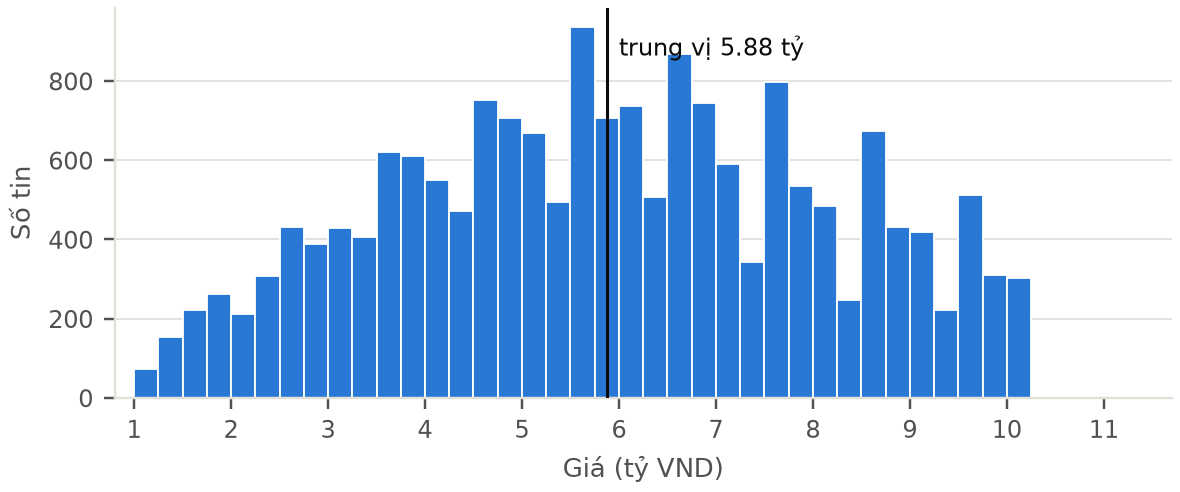
\includegraphics[width=\textwidth]{IMG/eda_price_dist.png}
\caption{Phân bố giá rao trên tập train (bước 0.25~\ty)}
\end{figure}

Giá có trung vị 5.88~\ty, trung bình 5.87~\ty, độ lệch chuẩn 2.21~\ty{} và độ lệch (skewness) gần 0
($-0.02$). Đây là dấu hiệu bất thường: giá bất động sản thực tế gần như luôn lệch phải với đuôi dài ở
phân khúc cao cấp. Phân bố cân đối và bị chặn gọn trong 1--11.5~\ty{} cho thấy nguồn dữ liệu đã lọc tin
theo khoảng giá. Diện tích có trung vị 56~\mtwo{} (từ 4 đến 595~\mtwo), còn đơn giá có trung vị 103~\trm{}
với 90\% giá trị trong khoảng 28--206~\trm.

\begin{figure}[H]
\centering
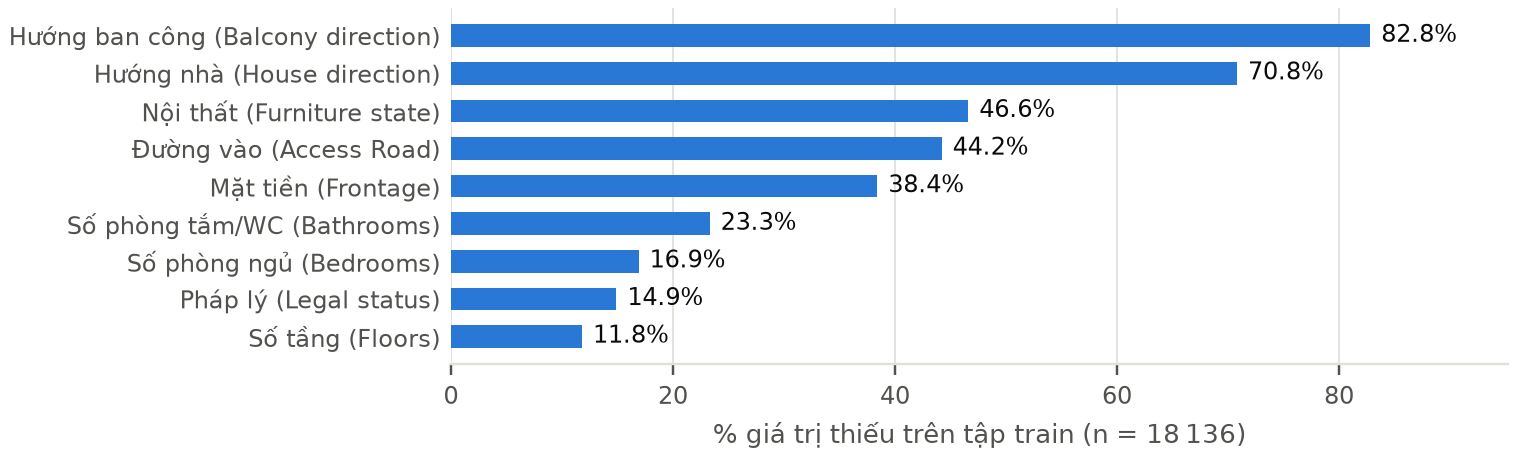
\includegraphics[width=0.92\textwidth]{IMG/eda_missing.png}
\caption{Tỷ lệ thiếu theo trường trên tập train}
\end{figure}

Hai trường hướng nhà, hướng ban công thiếu trên 70\%; nội thất, đường vào, mặt tiền thiếu 38--47\%.
Các trường ``mềm'' bị bỏ trống nhiều nhất, khớp với cơ chế người đăng tin chỉ điền những gì họ cho là
quan trọng.

\subsection{Quan hệ giữa các biến}

\begin{table}[H]
\centering
\small
\caption{Tương quan hạng Spearman giữa biến số và giá (tập train, bỏ dòng thiếu theo cặp)}
\begin{tabular}{@{}L{0.30\textwidth}L{0.12\textwidth}L{0.14\textwidth}L{0.34\textwidth}@{}}
\toprule
\textbf{Biến} & \textbf{n} & \textbf{$\rho$ với giá} & \textbf{Nhận xét} \\
\midrule
Số phòng tắm/WC (\texttt{Bathrooms}) & 13\,908 & 0.462 & Mạnh nhất trong nhóm biến số \\
Số phòng ngủ (\texttt{Bedrooms}) & 15\,077 & 0.425 & Đi cùng diện tích sàn \\
Số tầng (\texttt{Floors}) & 15\,991 & 0.325 & Nhà phố nhiều tầng giá cao hơn \\
Đường vào (\texttt{Access Road}) & 10\,126 & 0.245 & Ngõ rộng, ô tô vào được \\
Diện tích (\texttt{Area}) & 18\,136 & 0.193 & Yếu hơn kỳ vọng (xem IV.3) \\
Mặt tiền (\texttt{Frontage}) & 11\,177 & 0.112 & Yếu \\
\midrule
Diện tích với \textit{đơn giá} & 18\,136 & $-0.697$ & Nhà càng rộng, đơn giá càng thấp \\
\bottomrule
\end{tabular}
\end{table}

Với biến phân loại, nhóm dùng tỷ số tương quan $\eta^2$ (tỷ lệ phương sai của giá được giải thích bởi
trung bình từng nhóm). Cặp tỉnh + quận giải thích 24.9\% phương sai tổng giá và 61.8\% phương sai đơn giá;
tình trạng nội thất 3.7\%; hướng nhà 0.5\%; pháp lý gần 0\%.

\subsection{Khác biệt theo vị trí và diện tích}

\begin{figure}[H]
\centering
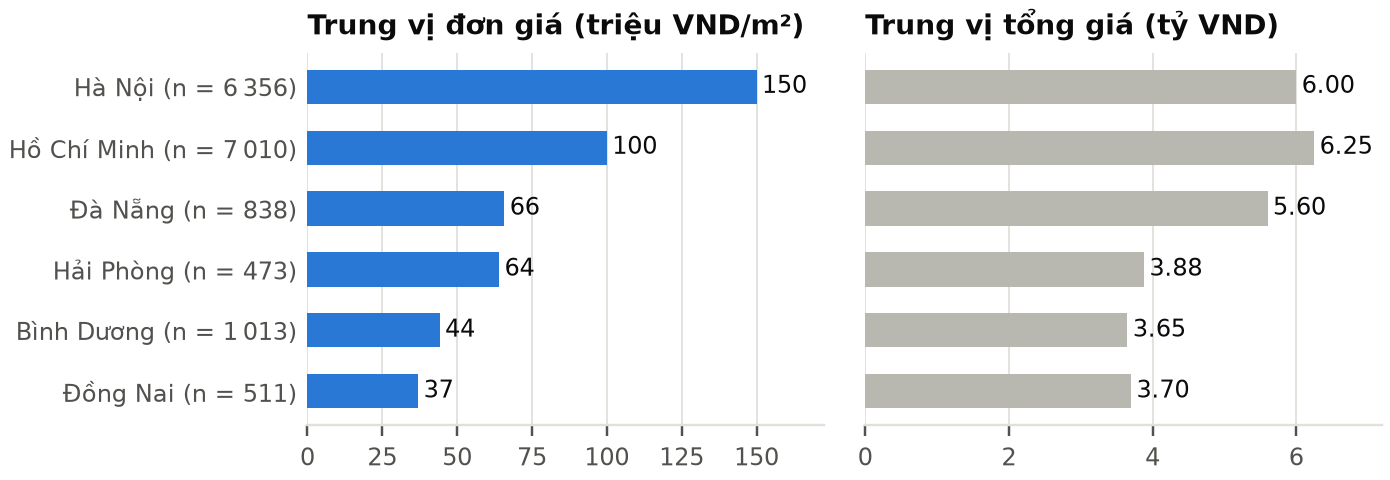
\includegraphics[width=0.86\textwidth]{IMG/eda_city.png}
\caption{Đơn giá và tổng giá theo 6 tỉnh/thành nhiều tin nhất (trung vị, tập train)}
\end{figure}

Đơn giá ở Hà Nội (150~\trm) gấp 4 lần Đồng Nai (37~\trm), nhưng tổng giá chỉ chênh 1.6 lần: người mua ở
Hà Nội nhận diện tích nhỏ hơn hẳn (trung vị 40~\mtwo{} so với 100~\mtwo). Nói cách khác, vị trí quyết định
\textit{đơn giá}, còn diện tích ``co giãn'' để tổng giá vừa với khả năng chi trả.

\begin{figure}[H]
\centering
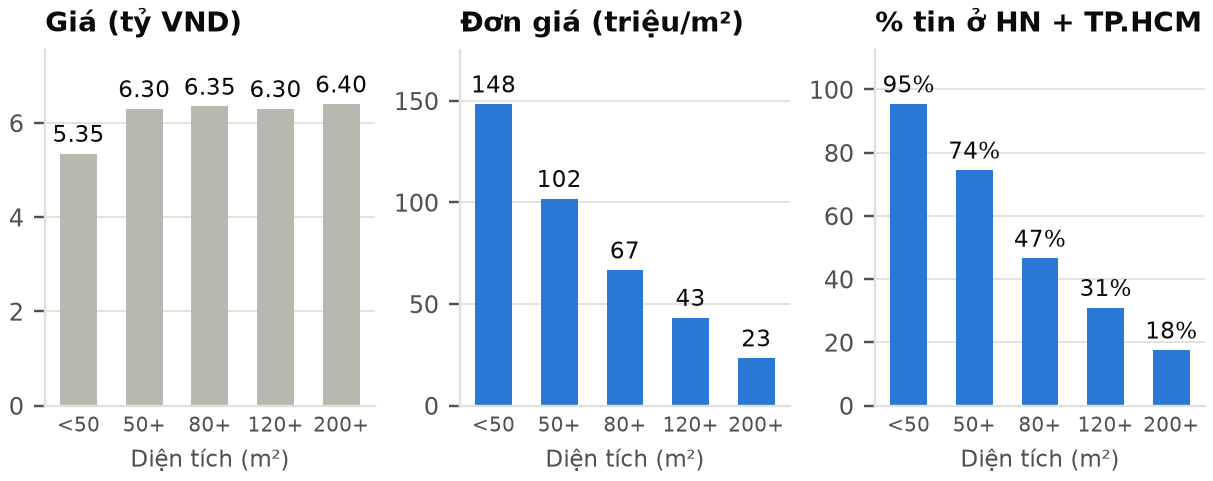
\includegraphics[width=0.92\textwidth]{IMG/eda_area_bins.png}
\caption{Theo nhóm diện tích (\mtwo; ``50+'' nghĩa là 50 đến dưới 80, ...): tổng giá trung vị gần như
đi ngang, đơn giá giảm mạnh và tỷ lệ tin ở Hà Nội + TP.HCM giảm theo}
\end{figure}

Từ 50~\mtwo{} trở lên, tổng giá trung vị đứng yên quanh 6.3--6.4~\ty{} dù diện tích tăng gấp bốn. Cùng lúc,
tỷ lệ tin ở Hà Nội và TP.HCM giảm từ 95\% (nhóm dưới 50~\mtwo) xuống 18\% (nhóm từ 200~\mtwo). Diện tích
lớn không làm giá cao hơn vì nhà diện tích lớn \textit{chỉ lọt vào khoảng 1--11.5~\ty{} khi nằm ở vùng giá rẻ}.

\subsection{Kiểm chứng giả thuyết}

\begin{table}[H]
\centering
\footnotesize
\caption{Kết quả kiểm chứng giả thuyết (tập train)}
\begin{tabular}{@{}L{0.05\textwidth}L{0.20\textwidth}L{0.27\textwidth}L{0.14\textwidth}L{0.23\textwidth}@{}}
\toprule
\textbf{ID} & \textbf{Phương pháp} & \textbf{Kết quả} & \textbf{Effect size} & \textbf{Kết luận} \\
\midrule
H1 & Kruskal--Wallis, $\eta^2$ trên đơn giá & 302 nhóm tỉnh--quận, $p < 10^{-300}$ & $\eta^2 = 0.618$ (lớn) & \textbf{Chấp nhận}: vị trí quyết định đơn giá. \\
H2 & Spearman \texttt{Area}--\texttt{Price} & $\rho = 0.193$; giá đi ngang từ 50~\mtwo{} & Nhỏ & \textbf{Bác bỏ ở mức toàn bộ dữ liệu}; chỉ đúng khi cố định vị trí (mục VII.3). \\
H3 & Mann--Whitney, có sổ vs HĐMB & Trung vị 5.85 vs 6.00~\ty; $p = 0.88$ & Cliff's $\delta = 0.004$ & \textbf{Bác bỏ} với tổng giá. \\
H4 & Spearman & \texttt{Bathrooms} 0.46; \texttt{Floors} 0.33 & Trung bình & \textbf{Chấp nhận}. \\
H5 & Kruskal--Wallis, 8 hướng & $p = 0.0009$; trung vị 5.05--5.60~\ty & $\eta^2 = 0.005$ & \textbf{Bác bỏ về thực tiễn}: có ý nghĩa thống kê nhưng hiệu ứng không đáng kể. \\
H6 & Mann--Whitney, Full vs Basic & Trung vị 6.20 vs 5.00~\ty; $p < 10^{-78}$ & Cliff's $\delta = 0.233$ & \textbf{Chấp nhận yếu}; biến mất khi có các biến khác (VII.3). \\
\bottomrule
\end{tabular}
\end{table}

\begin{warnbox}[Tương quan không phải nhân quả]
Nhà có sổ có \textit{đơn giá} cao gấp đôi nhà hợp đồng mua bán (106.6 so với 52.9~\trm, Cliff's $\delta = 0.54$),
nhưng không thể kết luận ``có sổ làm giá tăng gấp đôi''. Tin hợp đồng mua bán tập trung ở dự án vùng ven
(Đồng Nai, Hưng Yên, Bình Dương chiếm 34\%) với diện tích trung vị 100~\mtwo: vị trí và loại hình nhà là biến
thứ ba giải thích phần lớn khác biệt. Tương tự, nội thất đầy đủ đi cùng nhà nhỏ nội đô, nên hiệu ứng của
nội thất lẫn với hiệu ứng vị trí.
\end{warnbox}

%=====================================================================
\section{Preprocessing \& Feature Engineering}
%=====================================================================

\subsection{Tiền xử lý}

Mọi bước tiền xử lý nằm trong một \texttt{Pipeline} của scikit-learn và được fit lại trong từng fold, nên
không có thống kê nào (trung bình, mode, danh mục) được học từ phần dữ liệu dùng để chấm điểm.

\begin{enumerate}
    \item \textbf{Chuẩn hóa địa danh:} Unicode NFC, gộp khoảng trắng, bỏ dấu chấm cuối cho \texttt{City},
          \texttt{District}. Trên Random Forest, MAE validation của 120 dòng đổi tên giảm từ 1.030 xuống
          0.853~\ty.
    \item \textbf{Biến số:} chuẩn hóa (StandardScaler) rồi điền thiếu bằng trung bình. Nhóm đã so sánh trên
          validation: mean tốt hơn median (MAE 1.0188 so với 1.0212), tốt hơn KNN với $k = 3, 5, 15$
          (1.0237--1.0254) và thêm cờ thiếu không cải thiện (1.0236).
    \item \textbf{Biến phân loại:} điền mode rồi One-Hot (\texttt{handle\_unknown="ignore"} để quận mới
          không làm lỗi pipeline). Gán nhãn riêng \texttt{\_\_MISSING\_\_} cho ô thiếu cho kết quả kém hơn mode
          (1.0219 so với 1.0175). Sau mã hóa có 388 cột.
\end{enumerate}

\subsection{Feature Engineering theo domain}

\begin{table}[H]
\centering
\small
\caption{Các đặc trưng được tạo thêm hoặc đã thử}
\begin{tabular}{@{}L{0.18\textwidth}L{0.25\textwidth}L{0.29\textwidth}L{0.18\textwidth}@{}}
\toprule
\textbf{Đặc trưng} & \textbf{Cách tính} & \textbf{Ý nghĩa theo domain} & \textbf{Trạng thái} \\
\midrule
\texttt{City}, \texttt{District} & Tách \texttt{Address} theo dấu phẩy, lấy 2 phần cuối & Đại diện đơn giá đất khu vực (H1) & Dùng \\
Địa danh chuẩn hóa & NFC, bỏ dấu chấm, khoảng trắng & Gộp các biến thể của cùng một nơi & Dùng \\
Cờ thiếu dữ liệu & \texttt{isna()} cho 3 biến số & ``Không khai báo'' có thể mang thông tin & Đã thử, bỏ \\
Nhãn \texttt{\_\_MISSING\_\_} & Danh mục riêng cho ô trống & Như trên, cho biến phân loại & Đã thử, bỏ \\
Đơn giá/m\textsuperscript{2} & \texttt{Price / Area} & Thước đo của môi giới & Chỉ dùng cho EDA (rò rỉ nhãn) \\
\texttt{City\_District} & Ghép tỉnh và quận & Phân biệt quận trùng tên giữa các tỉnh & Kế hoạch \\
\bottomrule
\end{tabular}
\end{table}

\begin{codebox}[title={Pipeline tiền xử lý dùng chung cho các mô hình cây}, breakable]
import re
import unicodedata
import pandas as pd
from sklearn.compose import ColumnTransformer
from sklearn.impute import SimpleImputer
from sklearn.pipeline import Pipeline
from sklearn.preprocessing import (FunctionTransformer, OneHotEncoder,
                                   StandardScaler)

NUM = ["Area", "Frontage", "Access Road",
       "Floors", "Bedrooms", "Bathrooms"]
CAT = ["House direction", "Balcony direction", "Legal status",
       "Furniture state", "City", "District"]

def normalize_location_frame(X):
    # Chuan hoa ten dia phuong: NFC, gop khoang trang, bo dau cham cuoi
    X = X.copy()
    def norm(v):
        if pd.isna(v):
            return v
        v = unicodedata.normalize("NFC", str(v))
        return re.sub(r"\s+", " ", v).strip().rstrip(".").strip()
    for col in ["City", "District"]:
        X[col] = X[col].map(norm)
    return X

# So: chuan hoa roi dien mean; phan loai: dien mode roi One-Hot
num_pipe = Pipeline([("scaler", StandardScaler()),
                     ("imputer", SimpleImputer())])
cat_pipe = Pipeline([("imputer", SimpleImputer(strategy="most_frequent")),
                     ("onehot", OneHotEncoder(handle_unknown="ignore"))])

preprocessing = Pipeline([
    ("normalize_location", FunctionTransformer(normalize_location_frame)),
    ("columns", ColumnTransformer([("num", num_pipe, NUM),
                                   ("cat", cat_pipe, CAT)])),
])
\end{codebox}

\subsection{Chia tập dữ liệu}

Mỗi dòng là một căn nhà riêng và mục tiêu là ước lượng cho căn nhà khác trong cùng bối cảnh, không dự báo
tương lai, nên nhóm chia ngẫu nhiên với \texttt{seed = 42} và cố định từ đầu dự án:

\begin{table}[H]
\centering
\small
\caption{Giao thức chia dữ liệu}
\begin{tabular}{@{}L{0.18\textwidth}L{0.10\textwidth}L{0.10\textwidth}L{0.52\textwidth}@{}}
\toprule
\textbf{Tập} & \textbf{Tỷ lệ} & \textbf{Số dòng} & \textbf{Vai trò} \\
\midrule
Train & 60\% & 18\,136 & Fit tiền xử lý và mô hình; 3-fold CV cố định để chọn mô hình, tham số \\
Validation & 15\% & 4\,535 & So sánh nhanh ở giai đoạn khám phá, early stopping thử nghiệm \\
Calibration & 10\% & 3\,023 & Hiệu chỉnh khoảng dự đoán sau khi khóa mô hình (chưa dùng) \\
Test & 15\% & 4\,535 & Đánh giá cuối một lần duy nhất (chưa dùng) \\
\bottomrule
\end{tabular}
\end{table}

Bốn tập không giao nhau theo \texttt{row\_id} và được lưu thành file; khi sửa dữ liệu, nhóm tạo phiên bản
mới (\texttt{splits\_v2}) nhưng giữ nguyên thành viên từng tập để các kết quả so sánh được với nhau.

%=====================================================================
\section{Insights: Rút Ra Được Gì Từ Data?}
%=====================================================================

\subsection{Tổng hợp phát hiện chính}

\begin{table}[H]
\centering
\footnotesize
\caption{Các phát hiện chính từ data}
\begin{tabular}{@{}L{0.03\textwidth}L{0.17\textwidth}L{0.20\textwidth}L{0.20\textwidth}L{0.17\textwidth}L{0.08\textwidth}@{}}
\toprule
\textbf{\#} & \textbf{Phát hiện} & \textbf{Bằng chứng} & \textbf{Giải thích theo domain} & \textbf{Hành động} & \textbf{Độ tin cậy} \\
\midrule
1 & Vị trí quyết định đơn giá & $\eta^2 = 0.62$ trên đơn giá; HN 150 vs Đồng Nai 37~\trm & Giá đất theo khu vực là thành phần lớn nhất của giá nhà & Bắt buộc nhập tỉnh và quận trong app & Cao \\
2 & ``Nghịch lý diện tích'' & Giá đi ngang 6.3~\ty{} từ 50~\mtwo; $\rho(\text{diện tích}, \text{đơn giá}) = -0.70$ & Dữ liệu chỉ giữ 1--11.5~\ty: nhà rộng chỉ lọt vào nếu ở vùng rẻ & Không đọc diện tích tách khỏi vị trí & Cao \\
3 & Kết cấu quan trọng hơn diện tích đơn lẻ & $\rho$ WC 0.46, tầng 0.33 so với diện tích 0.19 & Nhà phố xây cao bù đất nhỏ; số tầng/WC đo diện tích sàn & Hỏi số tầng, WC; cảnh báo khi bỏ trống & Trung bình \\
4 & Pháp lý không làm khác tổng giá & $\delta = 0.004$, $p = 0.88$ & ``Hợp đồng mua bán'' là nhà dự án vùng ven, diện tích lớn & Không coi ``có sổ'' là điểm cộng giá độc lập & Trung bình \\
5 & Mô hình kéo giá về trung bình & Nhà $< 3$ tỷ bị đoán cao +0.97; nhà $\geq 9$ tỷ bị đoán thấp $-1.74$ & Thiếu thông tin chi tiết (vị trí trong quận, chất lượng) & Hiện khoảng giá và cảnh báo ở hai đầu & Cao \\
6 & Hướng nhà, nội thất gần như không đóng góp & Permutation importance $< 0.01$~\ty & Yếu tố phụ, lẫn với vị trí & Để là trường tùy chọn & Cao \\
\bottomrule
\end{tabular}
\end{table}

\subsection{Phát hiện bất ngờ và giả thuyết bị bác bỏ}

\textbf{Nghịch lý diện tích (H2).} Kỳ vọng ban đầu là ``nhà càng rộng càng đắt''. Ở mức toàn bộ dữ liệu,
điều này gần như không đúng: tương quan chỉ 0.19 và tổng giá đi ngang từ 50~\mtwo. Nguyên nhân là
\textit{selection bias} do nguồn chỉ giữ tin 1--11.5~\ty: một căn 200~\mtwo{} ở nội đô Hà Nội có giá vượt xa
11.5~\ty{} nên không có mặt trong dữ liệu; căn 200~\mtwo{} còn lại thường ở Bình Dương, Đồng Nai. Khi giữ
vị trí cố định, diện tích lại là đặc trưng quan trọng nhất của mô hình (mục VII.3). Đây là trường hợp
điển hình của nghịch lý Simpson: quan hệ trong từng nhóm khác với quan hệ khi gộp các nhóm.

\textbf{Pháp lý (H3) và phong thủy (H5).} Hai yếu tố được bàn nhiều khi mua nhà lại gần như không
giải thích được tổng giá trong dữ liệu này. Với pháp lý, khác biệt đơn giá có thật nhưng bị nhiễu bởi
vị trí và loại hình nhà; dữ liệu không có biến ``nhà dự án / nhà thổ cư'' để tách hai hiệu ứng. Với hướng
nhà, khác biệt trung vị giữa các hướng (5.05--5.60~\ty) nhỏ hơn nhiều so với độ biến động trong từng hướng.

\subsection{Nhóm, mẫu hình và phân khúc}

\begin{table}[H]
\centering
\small
\caption{Phân khúc theo vị trí và diện tích (tập train; sai số từ dự đoán out-of-fold của XGBoost)}
\begin{tabular}{@{}L{0.30\textwidth}L{0.08\textwidth}L{0.12\textwidth}L{0.14\textwidth}L{0.10\textwidth}L{0.12\textwidth}@{}}
\toprule
\textbf{Phân khúc} & \textbf{n} & \textbf{Giá (tỷ)} & \textbf{Đơn giá (tr/m\textsuperscript{2})} & \textbf{MAE} & \textbf{MdAPE} \\
\midrule
Nhà nhỏ Hà Nội ($< 50$~\mtwo) & 4\,807 & 5.68 & 158 & 0.93 & 13.1\% \\
Nhà phố Hà Nội (50--100~\mtwo) & 1\,453 & 7.60 & 129 & 1.20 & 12.9\% \\
Nhà nhỏ TP.HCM ($< 50$~\mtwo) & 2\,027 & 4.60 & 130 & 0.78 & 13.1\% \\
Nhà phố TP.HCM (50--100~\mtwo) & 4\,177 & 6.59 & 99 & 0.95 & 11.4\% \\
Nhà lớn TP.HCM ($\geq 100$~\mtwo) & 806 & 7.70 & 62 & 1.17 & 12.4\% \\
Tỉnh khác (50--100~\mtwo) & 2\,513 & 4.30 & 59 & 0.93 & 14.8\% \\
Tỉnh khác ($\geq 100$~\mtwo) & 1\,926 & 5.50 & 38 & 1.19 & 17.2\% \\
\bottomrule
\end{tabular}
\end{table}

Có thể gọi tên bốn nhóm theo ngôn ngữ thị trường: \textit{nhà nhỏ Hà Nội} (đất nhỏ, đơn giá rất
cao), \textit{nhà phố TP.HCM} (nhóm đông nhất, mô hình dự đoán tốt nhất, MdAPE 11.4\%), \textit{nhà đất
vùng ven} (diện tích lớn, đơn giá thấp, sai số tương đối cao hơn) và \textit{nhà dự án chưa có sổ}
(545 tin, đơn giá 53~\trm). MAE tuyệt đối tăng theo giá trị căn nhà, nhưng sai số tương đối lớn nhất lại
nằm ở các tỉnh ngoài Hà Nội và TP.HCM, nơi mỗi quận có ít tin để mô hình học.

\subsection{Từ insight đến quyết định}

\begin{figure}[H]
\centering
\begin{tikzpicture}[
    box/.style={draw, rounded corners=2pt, minimum height=11mm, minimum width=26mm,
                align=center, font=\small, fill=brandblue!12},
    arr/.style={-{Stealth[length=2.2mm]}, thick}]
    \node[box] (a) {Giá rao này\\có hợp lý?};
    \node[box, right=7mm of a] (b) {Tin rao cùng\\khu vực, kết cấu};
    \node[box, right=7mm of b] (c) {Vị trí + diện tích\\+ số tầng chi phối};
    \node[box, right=7mm of c] (d) {Ước lượng kèm\\cảnh báo độ tin cậy};
    \draw[arr] (a)--(b);
    \draw[arr] (b)--(c);
    \draw[arr] (c)--(d);
\end{tikzpicture}
\caption{Chuỗi giá trị của báo cáo: từ câu hỏi của người mua đến con số có kèm điều kiện sử dụng}
\end{figure}

\begin{greenbox}[Một insight tốt phải trả lời được ba câu]
(1) \textbf{Bằng chứng:} tổng giá đi ngang quanh 6.3~\ty{} từ 50~\mtwo{} trong khi đơn giá giảm từ 148
xuống 23~\trm{} và tỷ lệ tin ở Hà Nội + TP.HCM giảm từ 95\% xuống 18\%. (2) \textbf{Cơ sở domain:} giá nhà
$\approx$ đơn giá đất khu vực $\times$ diện tích; dữ liệu lọc theo khoảng giá nên nhà rộng chỉ xuất hiện ở
vùng rẻ. (3) \textbf{Hành động:} không bao giờ so sánh giá hai căn chỉ theo diện tích; ứng dụng phải bắt
buộc nhập vị trí và từ chối ước lượng ngoài khoảng mà dữ liệu bao phủ.
\end{greenbox}

%=====================================================================
\section{Modeling}
%=====================================================================

\subsection{Problem Formulation}

Bài toán là hồi quy có giám sát trên dữ liệu bảng. Với mỗi căn nhà $i$ có vector đặc trưng $\mathbf{x}_i$
gồm 12 biến (6 số, 6 phân loại), mô hình học hàm $f$ sao cho
\[
    \hat{P}_i = f(\mathbf{x}_i), \qquad
    \mathrm{MAE} = \frac{1}{n}\sum_{i=1}^{n} \left| P_i - \hat{P}_i \right| ,
\]
trong đó $P_i$ là giá rao (\ty). MAE là metric chọn mô hình vì cùng đơn vị với giá và người dùng hiểu ngay
(``sai trung bình bao nhiêu tỷ''); RMSE theo dõi lỗi lớn; $R^2$ là tiêu chí nghiệm thu của dự án
($R^2 \geq 0.7$ trên tập test). Ràng buộc: chỉ dùng thông tin người dùng khai báo được lúc dự đoán; pipeline
phải chịu được trường bỏ trống và quận chưa từng thấy.

\subsection{Baseline và lựa chọn mô hình}

Nhóm đi từ đơn giản đến phức tạp. Giai đoạn đầu so sánh nhanh trên tập validation; sau đó chuyển sang
3-fold cross-validation trên tập train để có ước lượng ổn định hơn và dùng cho tinh chỉnh tham số.

\begin{table}[H]
\centering
\small
\caption{Giai đoạn khám phá: so sánh trên tập validation (\texttt{splits\_v1}, 4\,535 dòng). Ba mô hình
boosting dùng chính tập validation để dừng sớm nên điểm của chúng hơi lạc quan.}
\begin{tabular}{@{}L{0.30\textwidth}L{0.09\textwidth}L{0.09\textwidth}L{0.09\textwidth}L{0.30\textwidth}@{}}
\toprule
\textbf{Mô hình} & \textbf{MAE} & \textbf{RMSE} & \textbf{$R^2$} & \textbf{Ghi chú} \\
\midrule
Baseline: trung vị giá train (5.88 tỷ) & 1.825 & 2.190 & 0.000 & Mốc sàn \\
Hồi quy tuyến tính & 1.264 & 1.643 & 0.437 & Thiếu quan hệ phi tuyến \\
Ridge ($\alpha = 1$) & 1.256 & 1.624 & 0.450 & Điều chuẩn cải thiện rất ít \\
Random Forest (mặc định) & 1.024 & 1.388 & 0.598 & Train $R^2$ 0.935: overfit \\
CatBoost (3\,000 vòng) & 0.991 & 1.315 & 0.639 & Fit chậm nhất \\
LightGBM (early stopping) & 0.986 & 1.320 & 0.637 & Fit 3 giây \\
XGBoost (3\,000 vòng) & 0.981 & 1.327 & 0.633 & MAE thấp nhất \\
\bottomrule
\end{tabular}
\end{table}

\begin{figure}[H]
\centering
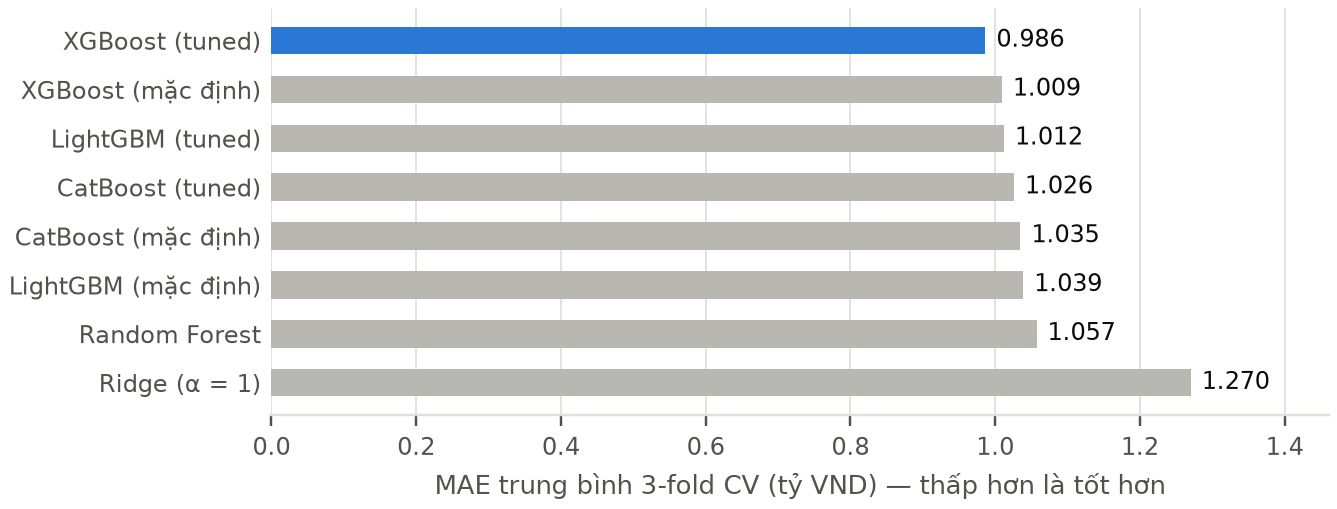
\includegraphics[width=\textwidth]{IMG/model_cv_mae.png}
\caption{So sánh 8 pipeline trên cùng 3 fold cố định của tập train (\texttt{splits\_v1})}
\end{figure}

Tinh chỉnh bằng grid search trên cùng 3 fold, chọn theo MAE trung bình; trong mỗi fold, số cây được chọn
bằng early stopping trên 15\% phần train của fold rồi refit, nên phần đánh giá không tham gia chọn số cây.

\begin{table}[H]
\centering
\small
\caption{Kết quả grid search lượt 1 (MAE 3-fold CV, \ty)}
\begin{tabular}{@{}L{0.14\textwidth}L{0.09\textwidth}L{0.47\textwidth}L{0.07\textwidth}L{0.07\textwidth}@{}}
\toprule
\textbf{Mô hình} & \textbf{Số cấu hình} & \textbf{Cấu hình chọn} & \textbf{Trước} & \textbf{Sau} \\
\midrule
Random Forest & 144 & \texttt{max\_features}=0.7, cây không giới hạn độ sâu & 1.057 & 1.057 \\
CatBoost & 27 & \texttt{depth}=8, \texttt{l2\_leaf\_reg}=3, \texttt{random\_strength}=2 & 1.035 & 1.026 \\
LightGBM & 36 & \texttt{num\_leaves}=63, \texttt{min\_child\_samples}=10 & 1.039 & 1.012 \\
XGBoost & 36 & \texttt{max\_depth}=9, \texttt{subsample}=0.8, \texttt{colsample\_bytree}=0.7 & 1.009 & \textbf{0.986} \\
\bottomrule
\end{tabular}
\end{table}

Hai ứng viên được giữ lại là \textbf{XGBoost} (sai số thấp nhất) và \textbf{LightGBM} (sai số gần tương
đương, huấn luyện nhanh hơn khoảng 8 lần). Sau khi sửa lỗi điền khuyết trước khi chia tập, cả hai được
huấn luyện lại trên \texttt{splits\_v2} và lưu checkpoint ngày 16/10/2026:

\begin{table}[H]
\centering
\small
\caption{Hai ứng viên trên \texttt{splits\_v2} (trung bình 3 fold)}
\begin{tabular}{@{}L{0.16\textwidth}L{0.10\textwidth}L{0.10\textwidth}L{0.10\textwidth}L{0.12\textwidth}L{0.28\textwidth}@{}}
\toprule
\textbf{Mô hình} & \textbf{MAE} & \textbf{RMSE} & \textbf{$R^2$} & \textbf{Train MAE} & \textbf{Số cây chọn (3 fold)} \\
\midrule
XGBoost & 0.984 & 1.319 & 0.645 & 0.553 & 738 / 1\,141 / 804 \\
LightGBM & 1.016 & 1.352 & 0.627 & 0.757 & 384 / 343 / 367 \\
\bottomrule
\end{tabular}
\end{table}

Sau khi bỏ giá trị điền sẵn, XGBoost không giảm chất lượng (MAE 0.986 $\rightarrow$ 0.984), cho thấy
điểm số trước đó không bị thổi phồng đáng kể bởi lỗi dữ liệu.

\begin{codebox}[title={Cấu hình XGBoost được chọn}]
from xgboost import XGBRegressor
from sklearn.pipeline import Pipeline

model = XGBRegressor(
    n_estimators=3000,      # tran tren; so cay that chon bang early stopping
    learning_rate=0.05,
    max_depth=9,
    min_child_weight=1,
    subsample=0.8,
    colsample_bytree=0.7,
    tree_method="hist",
    eval_metric="mae",
    random_state=42,
)
pipeline = Pipeline([("preprocessing", preprocessing), ("model", model)])

# Trong moi fold cua 3-fold CV:
#   1. tach 15% phan fit de chon so cay (dung sau 100 vong khong cai thien)
#   2. refit voi so cay da chon tren toan bo phan fit
#   3. cham MAE, RMSE, R2 tren phan assessment cua fold
\end{codebox}

\subsection{Mô hình học được điều gì?}

Nhóm đo \textit{permutation importance} trên chính phần đánh giá của từng fold: xáo trộn giá trị một đặc
trưng, giữ nguyên các đặc trưng khác, và đo MAE tăng thêm bao nhiêu. Cách đo này tính trên dữ liệu mô
hình chưa thấy và cho kết quả theo 12 biến gốc thay vì 388 cột One-Hot.

\begin{figure}[H]
\centering
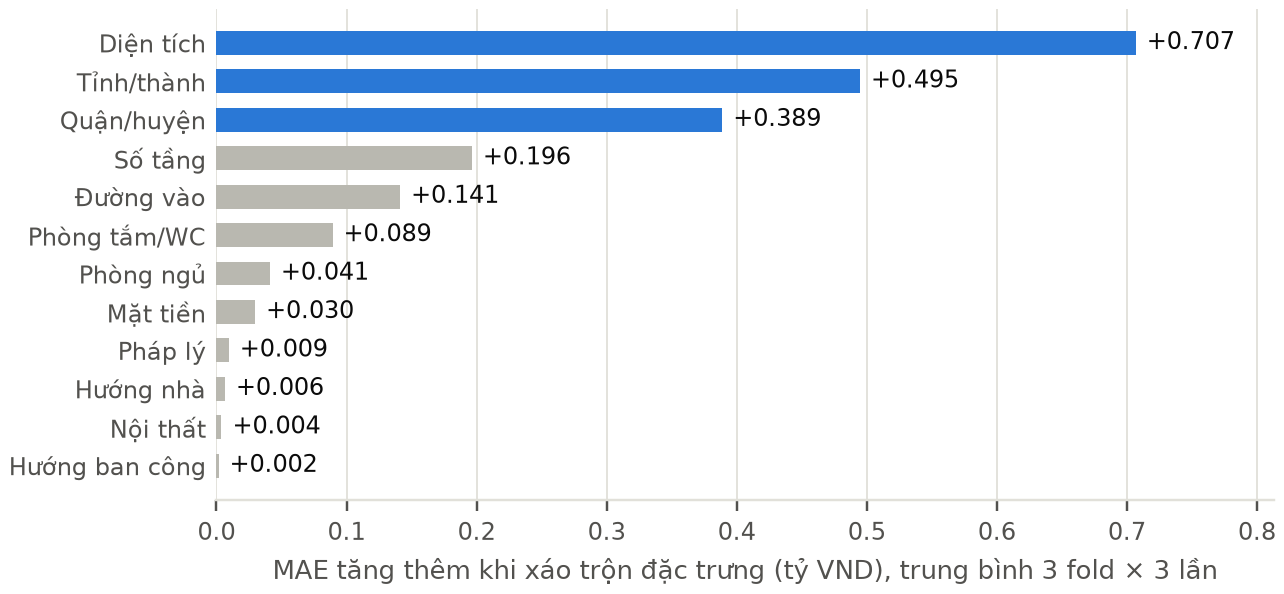
\includegraphics[width=\textwidth]{IMG/model_importance.png}
\caption{Permutation importance của XGBoost (\texttt{splits\_v2}, 3 fold $\times$ 3 lần xáo trộn)}
\end{figure}

\begin{itemize}
    \item \textbf{Vị trí là nhóm quan trọng nhất:} xáo trộn đồng thời tỉnh và quận làm MAE tăng 0.867~\ty,
          gần gấp đôi sai số hiện tại. Kết quả này đồng ý với H1 và phát hiện 1.
    \item \textbf{Diện tích đứng thứ hai về độ quan trọng riêng lẻ} (+0.707~\ty), dù tương quan đơn biến chỉ
          0.19. Mô hình học được đúng cơ chế ``giá $\approx$ đơn giá khu vực $\times$ diện tích'': diện tích
          chỉ có nghĩa khi đã biết vị trí. Đây là lời giải cho nghịch lý ở mục VI.2.
    \item \textbf{Kết cấu và hạ tầng}: số tầng (+0.196), đường vào (+0.141), phòng tắm (+0.089) xếp tiếp theo,
          khớp với H4 và với thực tế nhà phố nhiều tầng, ngõ ô tô vào được có giá cao hơn.
    \item \textbf{Pháp lý, hướng nhà, nội thất, hướng ban công} đều dưới 0.01~\ty: khi đã biết vị trí và kết
          cấu, các biến này gần như không thêm thông tin. Nội thất có khác biệt đơn biến ($\delta = 0.23$)
          nhưng khác biệt đó đã được giải thích bởi các biến khác.
\end{itemize}

\begin{notebox}[Quay về domain]
Thứ hạng của mô hình trùng với cách một môi giới có kinh nghiệm định giá: hỏi ``ở đâu'' trước, rồi ``bao
nhiêu mét'', rồi ``mấy tầng, ngõ rộng không''. Các yếu tố được nhắc nhiều trong tin rao như hướng nhà hay
nội thất hầu như không làm thay đổi giá rao trong khoảng 1--11.5~\ty.
\end{notebox}

%=====================================================================
\section{Evaluation}
%=====================================================================

\subsection{Chỉ số kỹ thuật}

Mọi con số trong mục này là dự đoán \textit{out-of-fold} trên 18\,136 dòng train của \texttt{splits\_v2}:
mỗi dòng được dự đoán bởi pipeline của fold không chứa dòng đó. Nhóm đã tái lập lại đúng MAE và $R^2$
từng fold đã lưu trong checkpoint trước khi phân tích. XGBoost đạt MAE 0.984~\ty, RMSE 1.319~\ty,
$R^2 = 0.645$; MAE từng fold nằm trong khoảng 0.978--0.992~\ty. Khoảng cách train/CV (0.55 so với 0.98~\ty)
cho thấy mô hình còn overfit, nhưng early stopping đã giữ sai số trên dữ liệu chưa thấy ổn định.

\begin{notebox}[Chưa phải kết quả nghiệm thu]
Tập test và calibration chưa được dùng. CV score đã được dùng để chọn cấu hình nên có thể lạc quan nhẹ.
Mục tiêu $R^2 \geq 0.7$ của dự án hiện \textbf{chưa đạt} trên CV (0.645); kết luận cuối cần một lần đánh
giá duy nhất trên test sau khi khóa mô hình.
\end{notebox}

\subsection{Chỉ số theo domain và giá trị thực tế}

Người mua không hỏi ``MAE bao nhiêu'' mà hỏi ``con số này lệch tối đa bao nhiêu phần trăm''. Bảng dưới
dịch kết quả sang các chỉ số đó và so với hai cách làm hiện tại, tính trên cùng các fold.

\begin{table}[H]
\centering
\small
\caption{Kết quả theo chỉ số domain (out-of-fold, 18\,136 căn)}
\begin{tabular}{@{}L{0.30\textwidth}L{0.12\textwidth}L{0.18\textwidth}L{0.12\textwidth}L{0.12\textwidth}@{}}
\toprule
\textbf{Chỉ số domain} & \textbf{Trung vị giá} & \textbf{Đơn giá quận $\times$ diện tích} & \textbf{LightGBM} & \textbf{XGBoost} \\
\midrule
\% căn có sai số $\leq 10\%$ & 19.0\% & 28.9\% & 37.8\% & \textbf{39.8\%} \\
\% căn có sai số $\leq 20\%$ & 36.8\% & 52.1\% & 65.4\% & \textbf{66.9\%} \\
Sai số tương đối trung vị (MdAPE) & 26.9\% & 19.0\% & 13.9\% & \textbf{13.3\%} \\
\% căn lệch quá 1 tỷ & 68.3\% & 51.8\% & 40.1\% & \textbf{38.1\%} \\
MAE (\ty) & 1.845 & 1.545 & 1.016 & \textbf{0.984} \\
\bottomrule
\end{tabular}
\end{table}

So với quy tắc đơn giá quận $\times$ diện tích, XGBoost nâng tỷ lệ căn được ước lượng trong $\pm 20\%$ từ
52\% lên 67\% và giảm sai số tương đối trung vị từ 19\% xuống 13\%. Với một căn 6~\ty, đó là chênh lệch
giữa sai khoảng 1.1~\ty{} và khoảng 0.8~\ty{} ở trường hợp điển hình. Tuy vậy, cứ ba căn vẫn có một căn
lệch hơn 20\%, nên con số chỉ nên dùng làm điểm tham chiếu.

\subsection{Error Analysis}

\begin{figure}[H]
\centering
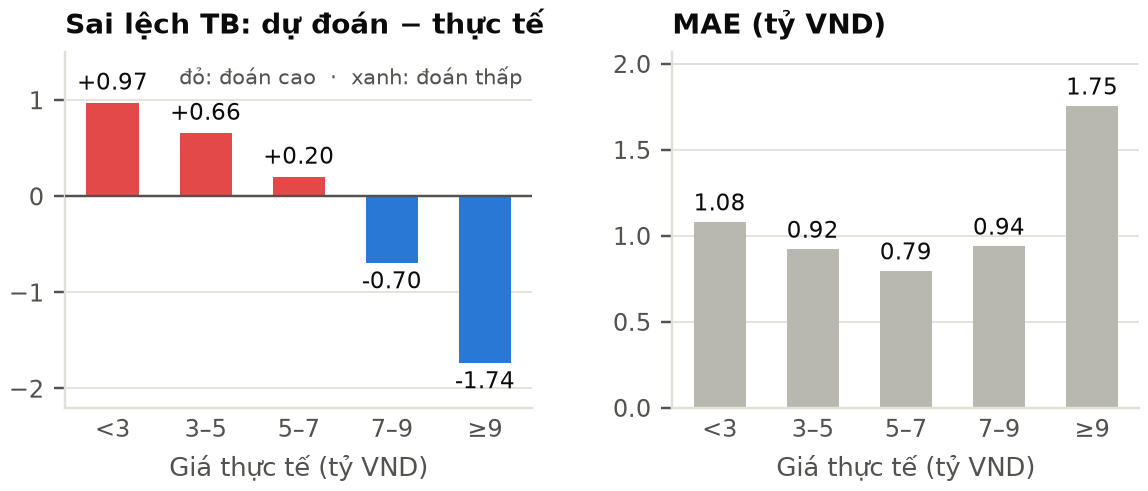
\includegraphics[width=\textwidth]{IMG/model_error_price.png}
\caption{Sai lệch trung bình (trái) và MAE (phải) của XGBoost theo nhóm giá thực tế (out-of-fold)}
\end{figure}

\begin{table}[H]
\centering
\small
\caption{Sai số XGBoost theo nhóm điều kiện (out-of-fold)}
\begin{tabular}{@{}L{0.36\textwidth}L{0.10\textwidth}L{0.10\textwidth}L{0.12\textwidth}L{0.14\textwidth}@{}}
\toprule
\textbf{Nhóm} & \textbf{n} & \textbf{MAE} & \textbf{Sai lệch TB} & \textbf{MdAPE} \\
\midrule
Quận có $\geq 100$ tin train & 15\,336 & 0.957 & $-0.01$ & 12.7\% \\
Quận có 30--99 tin & 1\,828 & 0.996 & $+0.02$ & 15.9\% \\
Quận có $< 30$ tin & 972 & 1.379 & $+0.31$ & 23.8\% \\
\midrule
Thiếu 0--2 trường tùy chọn & 6\,628 & 0.903 & $-0.02$ & 12.9\% \\
Thiếu 3--5 trường & 8\,179 & 0.968 & $+0.01$ & 13.0\% \\
Thiếu 6--9 trường & 3\,329 & 1.184 & $+0.07$ & 15.4\% \\
\midrule
Diện tích $< 50$~\mtwo & 7\,165 & 0.892 & $+0.02$ & 13.4\% \\
Diện tích $\geq 200$~\mtwo & 428 & 1.504 & $-0.06$ & 19.0\% \\
\bottomrule
\end{tabular}
\end{table}

Ba nhóm lỗi chính và nguyên nhân theo domain:

\begin{enumerate}
    \item \textbf{Kéo về trung bình ở hai đầu giá.} Căn dưới 3~\ty{} bị đoán cao trung bình 0.97~\ty, căn từ
          9~\ty{} bị đoán thấp 1.74~\ty. Hai căn cùng quận, cùng diện tích có thể chênh giá vì mặt đường hay
          ngõ sâu, nhà mới hay nhà cũ, những thông tin không có trong dữ liệu; mô hình vì thế dự đoán gần mức
          trung bình của nhóm. Dự đoán chỉ trải từ 0.14 đến 10.56~\ty, hẹp hơn khoảng giá thật.
    \item \textbf{Quận ít dữ liệu.} 972 căn ở các quận có dưới 30 tin train có MAE 1.38~\ty{} và bị đoán cao
          (+0.31~\ty): mô hình mượn mức giá của các quận đông dữ liệu, vốn đắt hơn.
    \item \textbf{Tin khai báo thiếu và nhà rất rộng.} Thiếu 6--9 trường làm MAE tăng 31\% so với tin khai báo
          gần đủ; nhà từ 200~\mtwo{} có MAE 1.50~\ty{} vì ít mẫu và đơn giá biến động mạnh ở vùng ven.
\end{enumerate}

\subsection{Kiểm chứng với chuyên gia domain}

Nhóm chưa có buổi phỏng vấn môi giới hoặc thẩm định viên. Đối chiếu gián tiếp: thứ hạng đặc trưng (vị trí,
diện tích, số tầng, đường vào) khớp với cách định giá theo phương pháp so sánh; chênh lệch đơn giá nội đô
và vùng ven phù hợp với hiểu biết chung về thị trường. Bước tiếp theo là cho 3--5 môi giới xem 20 ước lượng
ngẫu nhiên và ghi lại căn nào họ cho là sai, sai vì lý do gì.

%=====================================================================
\section{Application \& Recommendations}
%=====================================================================

\subsection{Cách sử dụng kết quả}

Nhóm đã xây dựng giao diện Streamlit (\nolinkurl{app/streamlit_app.py}) cho người dùng phổ thông, toàn bộ
tiếng Việt. Ứng dụng gọi mô hình qua một điểm duy nhất (\nolinkurl{app/core/model_interface.py}); hiện chạy ở
chế độ xem trước vì pipeline cuối chưa được khóa và xuất file.

\begin{figure}[H]
\centering
\begin{tikzpicture}[
    box/.style={draw, rounded corners=2pt, minimum height=11mm, minimum width=26mm,
                align=center, font=\small, fill=brandblue!12},
    arr/.style={-{Stealth[length=2.2mm]}, thick}]
    \node[box] (a) {Người dùng nhập\\12 thông tin};
    \node[box, right=7mm of a] (b) {Kiểm tra đầu vào\\\& chuẩn hóa địa danh};
    \node[box, right=7mm of b] (c) {Pipeline XGBoost\\ước lượng giá};
    \node[box, right=7mm of c] (d) {Hiện giá + khoảng\\+ cảnh báo};
    \draw[arr] (a)--(b);
    \draw[arr] (b)--(c);
    \draw[arr] (c)--(d);
\end{tikzpicture}
\caption{Quy trình ước lượng giá trong ứng dụng}
\end{figure}

Người dùng nhập vị trí và đặc điểm căn nhà; các trường có tỷ lệ thiếu cao trong dữ liệu (hướng nhà, hướng
ban công, nội thất) được để tùy chọn. Kết quả luôn hiển thị là \textit{ước lượng giá rao}, kèm đơn vị
\ty{} và các cảnh báo ở bảng dưới; không gọi là giá giao dịch hay giá thị trường.

\subsection{Khuyến nghị}

\begin{table}[H]
\centering
\footnotesize
\caption{Khuyến nghị dựa trên data}
\begin{tabular}{@{}L{0.22\textwidth}L{0.22\textwidth}L{0.14\textwidth}L{0.17\textwidth}L{0.14\textwidth}@{}}
\toprule
\textbf{Khuyến nghị} & \textbf{Căn cứ từ data} & \textbf{Người thực hiện} & \textbf{Tác động} & \textbf{Rủi ro} \\
\midrule
Bắt buộc nhập tỉnh và quận; gợi ý tên từ danh sách chuẩn hóa & Vị trí: importance 0.87~\ty; 26 biến thể tên tỉnh & Nhóm app & Giảm lỗi lớn nhất & Quận mới chưa có trong danh sách \\
Cảnh báo khi quận có $< 30$ tin hoặc giá dự đoán ngoài 1--11.5~\ty & MAE 1.38 ở quận ít tin; dự đoán thấp nhất 0.14~\ty & Nhóm app & Tránh tin nhầm con số yếu & Người dùng bỏ qua cảnh báo \\
Hiện khoảng giá thay vì một con số, hiệu chỉnh trên tập calibration & Sai lệch $+0.97$ / $-1.74$~\ty{} ở hai đầu & Nhóm model & Phản ánh đúng độ bất định & Khoảng quá rộng ở nhóm hiếm \\
Người mua: so giá rao với khoảng ước lượng, đặc biệt nhà diện tích lớn & Nghịch lý diện tích; MdAPE 13\% & Người dùng & Có cơ sở thương lượng & Thiếu thông tin chất lượng nhà \\
Người bán, môi giới: khai báo đủ số tầng, WC, đường vào & Thiếu 6--9 trường: MAE tăng 31\% & Người bán & Ước lượng sát hơn & Khai báo sai \\
\bottomrule
\end{tabular}
\end{table}

\subsection{Giám sát và cập nhật}

\begin{itemize}
    \item \textbf{Trước khi phát hành:} khóa cấu hình XGBoost, refit trên train + validation, hiệu chỉnh khoảng
          dự đoán trên calibration, đánh giá một lần trên test (MAE, RMSE, $R^2$, độ phủ của khoảng).
    \item \textbf{Drift dữ liệu đầu vào:} theo dõi phân bố tỉnh/quận, diện tích và tỷ lệ bỏ trống của người
          dùng so với tập train; tỷ lệ quận ``chưa từng thấy'' tăng là tín hiệu cần bổ sung dữ liệu.
    \item \textbf{Drift giá:} dữ liệu là ảnh chụp năm 2024; khi có tin rao mới, so trung vị đơn giá theo quận
          với dữ liệu cũ. Nếu lệch hơn 10\% ở các quận lớn, huấn luyện lại thay vì tiếp tục dùng mô hình cũ.
\end{itemize}

%=====================================================================
\section{Limitations \& Future Work}
%=====================================================================

\begin{itemize}
    \item \textbf{Giới hạn dữ liệu:} giá rao, không phải giá giao dịch; chỉ khoảng 1--11.5~\ty, nên mô hình
          không có cơ sở cho nhà rẻ hơn hoặc đắt hơn; 74\% tin ở Hà Nội và TP.HCM; một thời điểm năm 2024.
          Đơn vị của diện tích, mặt tiền, đường vào chưa được nguồn mô tả rõ.
    \item \textbf{Thông tin thiếu:} không có tọa độ, tên đường cụ thể, năm xây dựng, loại hình (nhà dự án/thổ cư,
          mặt phố/trong ngõ). Đây là nguyên nhân chính của hiện tượng kéo về trung bình.
    \item \textbf{Đánh giá chưa hoàn tất:} chưa đánh giá trên test, chưa hiệu chỉnh khoảng dự đoán, $R^2$ CV 0.645
          chưa đạt mục tiêu 0.7; chưa phỏng vấn chuyên gia domain.
    \item \textbf{Giả định chưa kiểm chứng:} mỗi dòng là một căn nhà riêng (202 dòng trùng thuộc tính chưa xác minh);
          mối quan hệ giữa các biến giữ nguyên khi thị trường thay đổi sau 2024.
\end{itemize}

\textbf{Hướng phát triển:}
\begin{enumerate}
    \item Thêm đặc trưng vị trí chi tiết hơn: \texttt{City\_District}, target encoding đơn giá theo quận có làm
          mượt cho quận ít tin, hoặc tọa độ khi có địa chỉ đầy đủ.
    \item Huấn luyện trên log giá hoặc dùng quantile regression để giảm kéo về trung bình và tạo khoảng dự đoán.
    \item Ensemble XGBoost + LightGBM, phân tích SHAP cho từng ước lượng để giải thích trong ứng dụng.
    \item Thu thập dữ liệu mới có ngày đăng để đo biến động giá theo thời gian; kiểm chứng với môi giới.
\end{enumerate}

%=====================================================================
\appendix
%=====================================================================
\section{Data Dictionary đầy đủ}

\begin{table}[H]
\centering
\small
\caption{Toàn bộ biến trong dữ liệu sau khi tách địa chỉ (\% thiếu trên 30\,229 dòng gốc)}
\begin{tabular}{@{}L{0.18\textwidth}L{0.11\textwidth}L{0.09\textwidth}L{0.38\textwidth}L{0.10\textwidth}@{}}
\toprule
\textbf{Biến} & \textbf{Kiểu} & \textbf{Đơn vị} & \textbf{Ý nghĩa, giá trị} & \textbf{\% thiếu} \\
\midrule
\texttt{Price} & Số thực & \ty & Tổng giá rao; 1.0--11.5 & 0.0 \\
\texttt{Area} & Số thực & \mtwo & Diện tích ghi trên tin; 3.1--595 & 0.0 \\
\texttt{Frontage} & Số thực & m & Mặt tiền; 1--77 (giá trị gốc) & 38.3 \\
\texttt{Access Road} & Số thực & m & Độ rộng đường vào; 1--85 & 44.0 \\
\texttt{Floors} & Số nguyên & tầng & 1--10 & 11.9 \\
\texttt{Bedrooms} & Số nguyên & phòng & 1--9 & 17.1 \\
\texttt{Bathrooms} & Số nguyên & phòng & 1--9 & 23.4 \\
\texttt{House direction} & Phân loại & -- & 8 hướng (Đông, Tây - Nam, ...) & 70.3 \\
\texttt{Balcony direction} & Phân loại & -- & 8 hướng & 82.6 \\
\texttt{Legal status} & Phân loại & -- & \texttt{Have certificate}, \texttt{Sale contract} & 14.9 \\
\texttt{Furniture state} & Phân loại & -- & \texttt{Full}, \texttt{Basic} & 46.7 \\
\texttt{City} & Phân loại & -- & Phần cuối của \texttt{Address}; 106 tên gốc & 0.0 \\
\texttt{District} & Phân loại & -- & Phần áp chót của \texttt{Address}; 341 tên gốc & 0.0 \\
\texttt{row\_id} & Số nguyên & -- & Khóa truy vết dòng; không phải đặc trưng & 0.0 \\
\bottomrule
\end{tabular}
\end{table}

\section{Reproducibility \& Code Structure}

\begin{itemize}
    \item \textbf{Seed:} 42 cho chia tập, fold CV, chia trong fold để early stopping và mô hình.
    \item \textbf{Phiên bản thư viện:} Python 3.14; numpy 2.5.3; pandas 3.0.6; scikit-learn 1.9.1; xgboost 3.4.1;
          lightgbm 4.7.0; catboost 1.2.10; joblib 1.6.0.
    \item \textbf{Dữ liệu:} \texttt{splits\_v2} được tạo lại từ \texttt{splits\_v1} bằng
          script \nolinkurl{src/preprocessing/repair_input_v2.py} đi kèm checkpoint (tham số
          \texttt{-{}-project-root} là thư mục repo); tập train có SHA-256 bắt đầu bằng
          \texttt{bcbc0634}, đã đối chiếu khớp với manifest của checkpoint.
    \item \textbf{Checkpoint:} \nolinkurl{models/candidates/milestone_v2_r2_2026-10-16/} chứa 3 pipeline CV của
          mỗi mô hình (không phải mô hình final), kèm manifest, chỉ số từng fold và mã tiền xử lý.
\end{itemize}

\begin{codebox}[title={Cấu trúc thư mục repo}, breakable]
AIQS-Real-Estate-Price-Prediction/
|-- data/
|   |-- vietnam_housing_dataset.csv   # du lieu goc, khong sua
|   |-- _v1.csv                        # sau khi tach dia chi
|   `-- processed/splits_v1/           # train/validation/calibration/test
|-- notebooks/
|   |-- cleandata_estate_aiqs.ipynb    # lam sach, tach Address
|   |-- 01_data_handoff_and_split.ipynb
|   |-- 02_baseline_models.ipynb       # Dummy, Linear, Random Forest
|   `-- 03_model_experiments.ipynb     # boosting, CV, grid search
|-- experiments/                       # ket qua CV va grid search (CSV)
|-- models/candidates/                 # checkpoint XGBoost, LightGBM
|-- app/
|   |-- streamlit_app.py               # giao dien nguoi dung
|   `-- core/                          # schema, validation, model_interface
|-- reports/application_report/        # bao cao nay: main.tex, def.tex,
|                                      #   title.tex, IMG/ (logo + hinh)
`-- README.md
\end{codebox}

\end{document}
